%!TEX root = ../../main.tex

\chapter{EDRICO}
<<<<<<< HEAD

The Proposed Processor design named \ac{EDRICO} implements a basic \ac{RV32I}
instruction set architecture. Besides the mandatory Zicsr extension no other
=======
\label{chapter:edrico}
The Proposed Processor design named Educational DHBW RISC-V Core (EDRICO) implements a basic RV32I
instruction set architecture. Besides the mandatory “Zicsr” extension no other
>>>>>>> 11e7a5a18fb89c84c3d44061ef46d9eba6d9893f
instruction set extensions are implemented. To keep the implementation simple and
straight-forward only one privilege mode (machine-mode) is implemented. This mode
allows full access to the processor and peripherals. Future versions could be
extended to implement supervisor- and user-mode.\\
The core is a simple \acf{SISD} processor without any pipeline or cache. The basic instruction cycle of fetch, decode, execute is performed for every instruction one at a time.\\
Figure \ref{fig:edricooverview} shows the full overview of the processor design:

\begin{figure}[H]
	\centering
	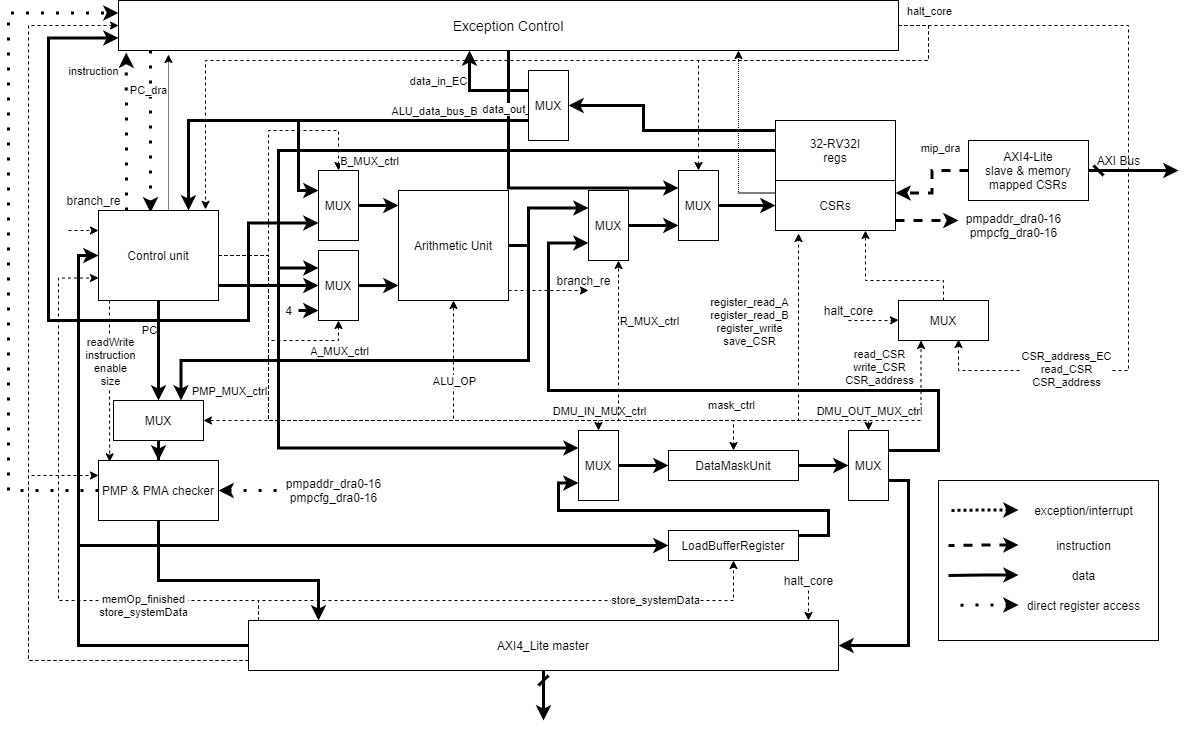
\includegraphics[width=150mm,scale=0.5]{datapath_EDRICO}
	\caption{EDRICO Overview}
	\label{fig:edricooverview}
\end{figure}

Its main components are the \textit{Exception Control}, \textit{Control Unit}, \ac{ALU},
\textit{Register Files}, \textit{PMP \& PMA checker} and the \ac{AXI}4 Interfaces. How these components interact with each other, in order to execute Instructions, is specified in the data path.
The following sections will describe each one of the components in more detail.

\section{Data Path}
The Data Path specifies how the data is passed through the Processor Core at run time. It therefore determines what registers are read and written at which clock cycle, what control signals need to be applied and how many cycles the instruction execution takes.\\
To run an instruction, it must be fetched, decoded and executed. Execution varies for different instructions.\\
To perform for example a load, the target address must be calculated and verified for possible access constraints. After successfully accessing the memory space, the obtained data is modified to satisfy the instruction specific formatting. 
A load half-word unsigned operation for instance must return a 32-Bit value by zero extending the loaded two bytes of data.\\
In case of a simple register-register addition, execution is found to be a lot simpler. Addition is performed inside the Arithmetic Logic Unit on two register values. The result is stored to the target register on the next falling clock edge.\\
With the end of the execute phase, the Programm Counter is updated. This ensures that the 32-Bit register always contains the address of the current instruction to be fetched, decoded and executed.  \\
Figure \ref{fig:datapath_generic} shows the different actions that are performed on each clock cycles during run time:

\begin{figure}[H]
	\centering
	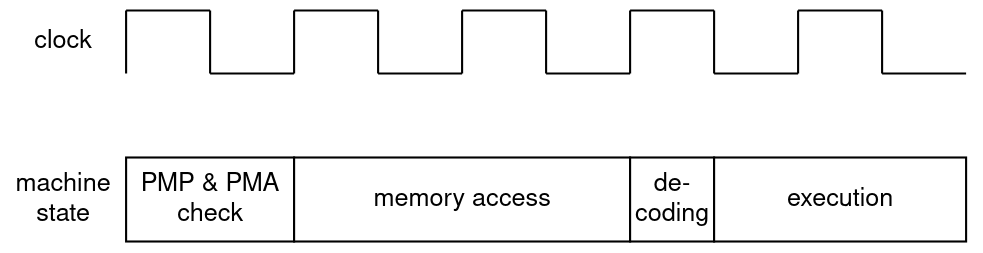
\includegraphics[width=150mm,scale=0.5]{DataPath}
	\caption{Generic Data Path}
	\label{fig:datapath_generic}
\end{figure}

Prior to memory access, the address must be checked for possible violations of the physical memory protection (PMP) and physical memory attribute (PMA) rules. Therefore the PC is passed to the PMP and PMA checker unit (see: \ref{fig:edricooverview}).\\
PMP and PMA checks are finished one clock cycle later, if an exception is generated, the trap is taken. Otherwise the data as well as the control signals are passed to the AXI4-Lite master.
The AXI4-Lite transfer will take multiple clock cycles. Its length can be increased by external factors, such as the memory to be accessed or the amount of data currently passing through the AXI-interconnect. To simplify the depiction in \ref{fig:datapath_generic} it is assumed to take only two clock cycles.\\
After successfully accessing the memory, decoding is performed in half a clock cycle. Decoding returns all the control signals of EDRICO set to the correct levels in order to perform the desired operation. Hence, no control signals do change during execution. This is desired since it will allow an easier pipelined implementation of a RISC-V core based on EDRICO.\\
Execution is displayed to take one and a half clock cycles. The registers are written at the falling clock cycle, one cycle after decoding started. Therefore execution is finished after only one clock cycle and not one and a half. Since the next instruction fetch is issued at a rising clock edge the machine must remain in execution state for an additional half clock cycle. \\
The fact that some registers are falling-edge and others rising-edge sensitive may seem a little bit disturbing at first glance. It is done to allow easier implementation and achieving of timing-closure during place and rout. If, for example, a critical path is found to be at the decode process, the duty cycle of the clock can be modified in order to achieve a higher possible clock frequency.

\clearpage
\section{Control Unit}
The \ac{CU} is the heart of the processor and controls the other parts of the processor depending on the input instruction. The CU is responsible for fetching instructions from the instruction memory, decode the bitstream and set the respective control signals for the other processor components. Due to the complexity of the CU, there are several sub-modules which together form the overall CU.
\subsection{Architecture and Design}
\label{CU_arch}
A general overview of the CU architecture is displayed in Figure \ref{fig:cuarchitecture}. 

\begin{figure}[H]
	\centering
	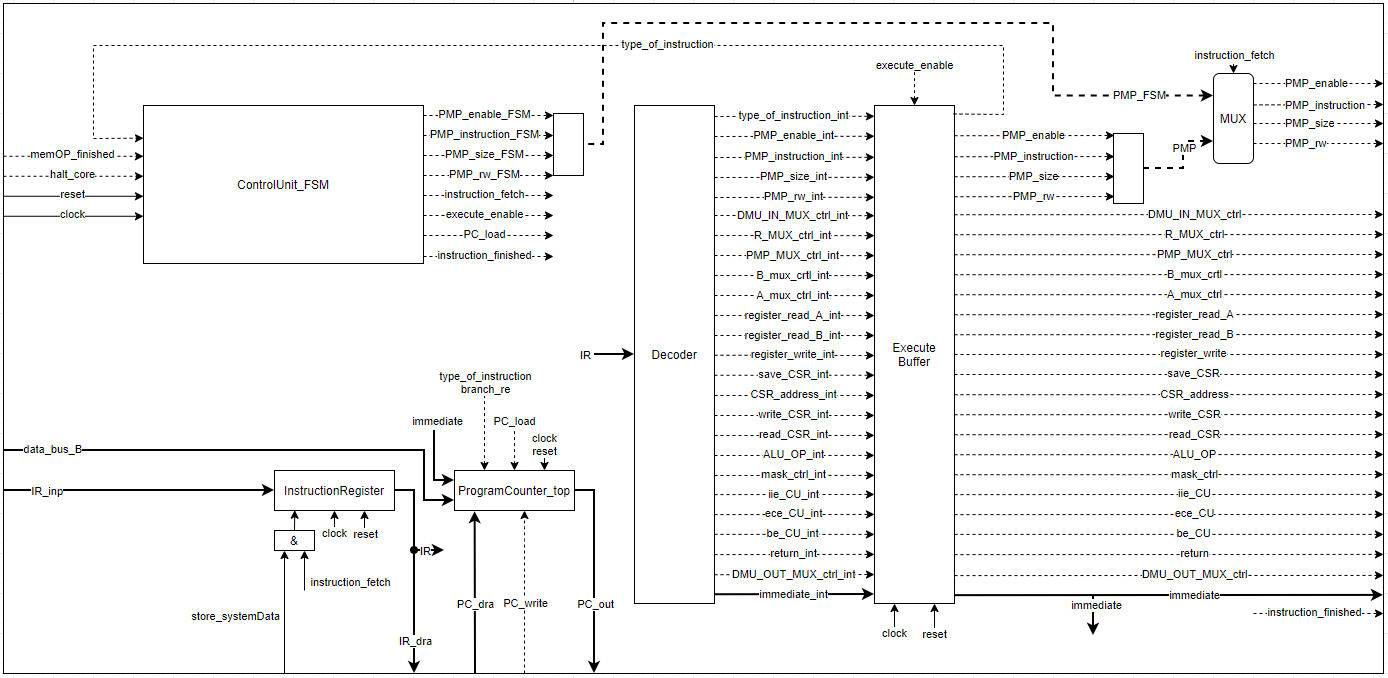
\includegraphics[width=\textwidth]{CU_architecture}
	\caption{Control Unit Architecture}
	\label{fig:cuarchitecture}
\end{figure}

To describe the functionality of the CU in more detail, every sub-module will be described closely.\\
Since the Control Unit is responsible for the whole processor, it is important to have a persistent and stable procedure for every instruction that shall be executed. The Control Unit \ac{FSM} is responsible for the correct clock timings which is important due to memory operations and the execution time of the other processor parts. The states and conditions of the FSM are displayed in Figure \ref{fig:cufsm}. 

\begin{figure}[H]
	\centering
	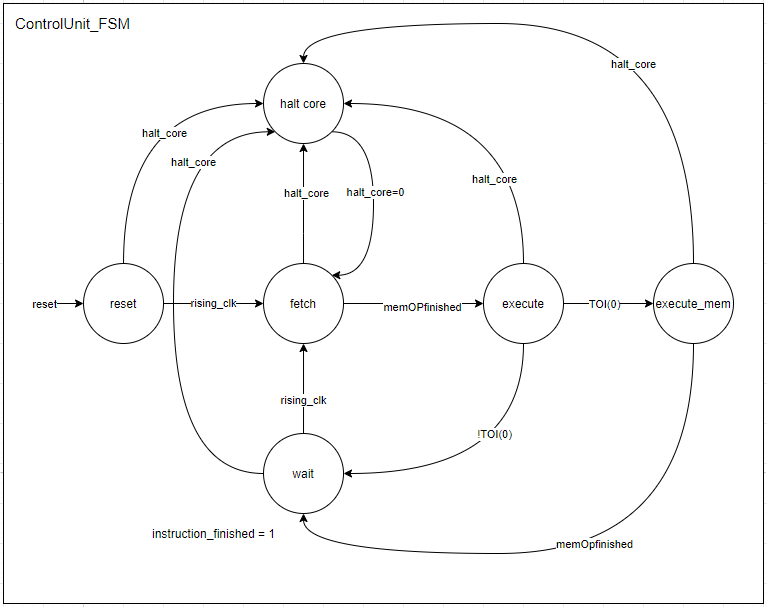
\includegraphics[width=\textwidth]{CU_FSM}
	\caption{Control Unit FSM overview}
	\label{fig:cufsm}
\end{figure}

Table \ref{tableFSM} shows a more detailed overview of the clock cycles and the corresponding actions and states:\\

\begin{table}[h]
\setlength\arrayrulewidth{2pt}	
\resizebox{\textwidth}{!}{
	\begin{tabular}{|c|c|l|l|}
		\hline
		\rowcolor{light-gray}
		\textbf{ClockCycle} & \textbf{Edge} & \textbf{Action} & \textbf{Signal} \\
		\hline
		1 & rising & pass the PC and enable PMP \& PMA checker with respective information &  \\
		\hline
		& falling & N/A &  \\
		\hline
		4 & rising & data is ready in instruction register - switch to execute state & \textit{memOPfinished} \& \textit{store\_systemData} is high \\
		\hline
		5 & rising & execution is started - if memory operation wait for another \textit{memOPfinished} flag, otherwise wait & \textit{execute\_enable} \\
		\hline
		x & rising & during memory operation: data loaded to buffer \textbackslash store transfer finished $\rightarrow$ wait state & \textit{memOPfinished} \& \textit{store\_systemData} is high \\
		\hline
		& falling & if load: store data form buffer to specified location &  \\
		\hline
		6 / x+1 & rising & go to \textit{fetch\_state} &  \\
		\hline
	\end{tabular}}
\caption{Timing of FSM}
\label{tableFSM}
\end{table}

During an execution cycle, the FSM controls the rest of the CU consisting of memory, decoding unit, PC control and the different multiplexers. To understand what the purpose of the different signals are, the other components of the Control Unit are described in the following sections.

After loading an instruction from the memory to the instruction register, the decoding process can begin. The responsible part for this process is the decoding unit which is described below.(Also visible in figure \ref{fig:cuarchitecture})\\
In this project the RISC-V RS32I instruction set is used which consists of 32-bit instruction words. The instruction words have a pre-defined structure and are divided into six instruction formats.
The instruction formats are shown in Figure \ref{fig:instrtypes}.

\begin{figure}[h]
	\centering
	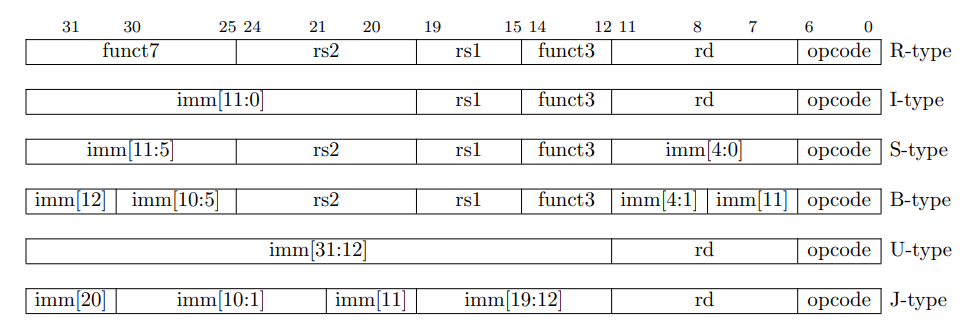
\includegraphics[width=\textwidth]{instr_types.png}
	\caption{RISC-V Instruction formats \cite{riscv}}
	\label{fig:instrtypes}
\end{figure}
The different instruction formats are useful for the decoding process since e.g. all LOAD instructions have the same structure and therefore, the effort to decode the 32-bit word can be reduced. Since the control signals are unique for every instruction and depending on the content of the 32-bit word, the decoder has to identify the encoded instruction, extract the information and respectively set the control signals, calculate immediates and control the multiplexers. A more detailed description of the decoding process can be found in section \ref{CU_impl}.\\
After the instruction is decoded, all output control signals are stable and ready to be fed through. Before leaving the CU, the \textit{Execute Buffer} (figure \ref{fig:cuarchitecture}) buffers the control signals. Once the FSM sets the \textit{execute\_enable} flag, the control signals are fed through. This buffer prevents the processor to confuse timing and clock cycles, or use signals which are not yet set correctly.\\
During an instruction execution, the program counter has to be incremented for the processor to know what instruction will follow. \textit{But} since there are several instructions that modify the program counter, a so called \textit{PC control} is designed. The PC control receives information from the decoder which consists of a 4 bit signal. The different instructions and the respective action as well as the respective control signal are shown in following table \ref{PCcontrol}:\clearpage

\begin{table}[h]
\setlength\arrayrulewidth{2pt}
	\resizebox{\textwidth}{!}{
		\begin{tabular}{|l|l|l|}
			\hline
			\rowcolor{light-gray}
			\textbf{Instruction} & \textbf{Action} & \textbf{Control Signal}\\
			\hline
			Default & No action required & \textbf{0000}\\
			\hline
			Branch & Depending on the result of branch operation, PC will be incremented respectively & \textbf{0010}\\
			\hline
			JAL & Target address obtained by adding current PC and immediate, rejump address stored in register & \textbf{0100}\\
			\hline
			JALR & Target address obtained by adding input register to immediate & \textbf{1000}\\
			\hline
		\end{tabular}}
	\label{PCcontrol}
	\caption{Program Counter control: Instructions and rAXIesulting actions}
\end{table}
For instructions which do not influence the program counter, the standard operation performs the \textbf{PC + 4} operation.

The instruction register displayed in figure \ref{fig:cuarchitecture} manages the instruction string coming from the memory.
All of these parts together form the Control Unit and are responsible for the correct execution of the instructions. The implementation of the sub-units in VHDL are described in the following section \ref{CU_impl}.\clearpage

\subsection{Implementation}
\label{CU_impl}
The implementation of the Control Unit is split up into multiple sub-implementations. As shown in figure \ref{fig:cuarchitecture} those sub-modules are the \textit{FSM, decoder, execute\_buffer, PC control and instruction register}. Since the implementation of the FSM is very similar to other FSM implementations in this project, the detailed description of a FSM in VHDL is found in the next chapters.\\
In this section the implementation of the decoder will be described more closely.
As already described in section \ref{CU_arch} the instructions can be separated in different instruction formats. To distinguish the different instructions, so-called \textit{instruction clusters} are created. These clusters sum up instructions which are encoded in the same instruction format or in general are similar.
The following table shows the different clusters and the corresponding instructions:
\begin{table}[h]
\setlength\arrayrulewidth{2pt}
	\centering
		\begin{tabular}{|l|l|}
			\hline
			\rowcolor{light-gray}
			\textbf{Cluster} & \textbf{Instructions}\\
		
			\hline
			LOAD & Load - Byte \textbackslash Halfword \textbackslash Word\\
			
			\hline
			STORE & Store - Byte \textbackslash Halfword \textbackslash Word\\
			
			\hline
			BRANCH & Different Branch Instructions (e.b. Branch if equal)\\
			
			\hline
			JALR & only JALR, since it has a unique instruction structure\\
			
			\hline
			JAL & only JAL, since it has a unique instruction structure\\
			
			\hline
			OP & All arithmetic instructions like ADD, SUB, shift and comparisons\\
			
			\hline
			OP-IMM & All arithmetic instructions performed with immediate\\
			\hline
			AUIPC & only AUIPC, since it has a unique instruction structure\\
			\hline
			LUI & only LUI, since it has a unique instruction structure\\
			\hline			
	\end{tabular}
	\label{instructioncluster}
	\caption{Decoding instruction clusters}
\end{table}


To determine the cluster for each instruction, a decoding procedure is implemented in VHDL based on structure visualized in figure \ref{fig:decode_structure}:

\begin{figure}[H]
	\centering
	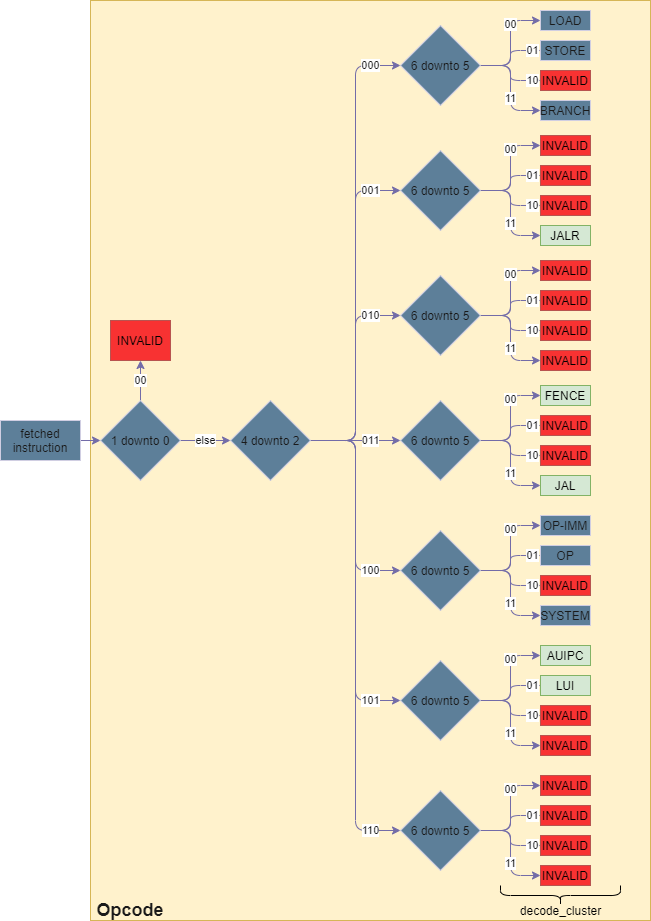
\includegraphics[width = 120mm]{Decode_Structure}
	\caption{Decoding Structure to determine instruction cluster}
	\label{fig:decode_structure}
\end{figure}
After determining the cluster, the VHDL code assigns all the outputs visible in figure \ref{fig:cuarchitecture} with the respective information. For a better understanding of the information extraction, figure \ref{fig:instruction_bits} shows how the 32-bit instruction word is split up (in this case for the \textit{OP} and \textit{OP-IMM} instructions.)
\begin{figure}[H]
	\centering
	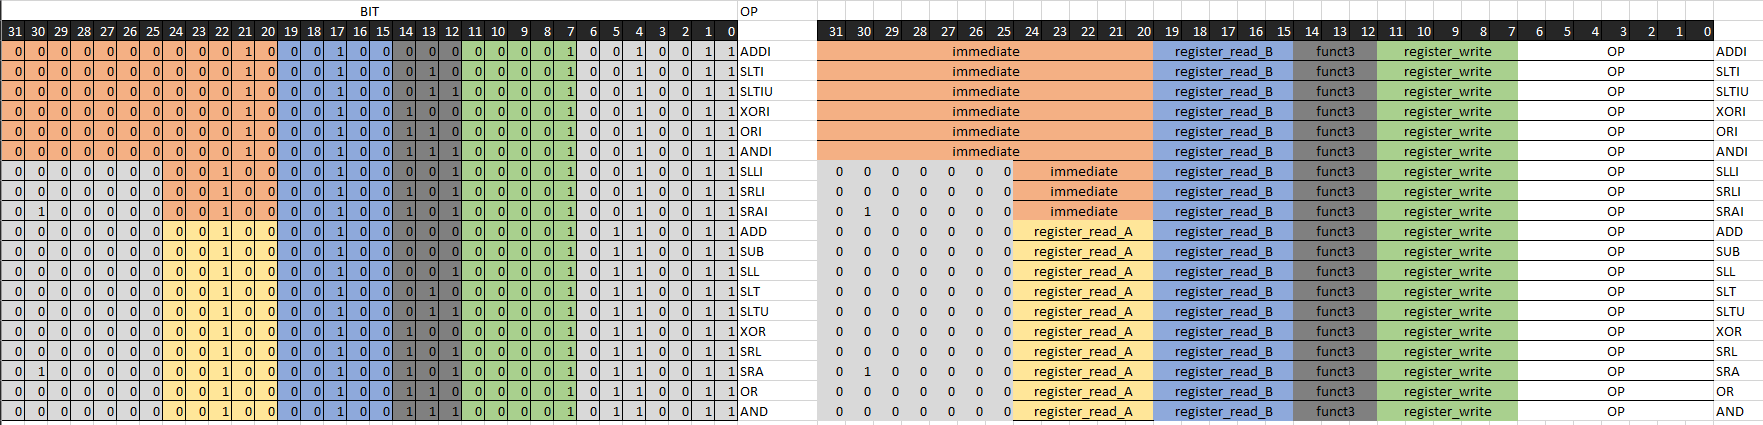
\includegraphics[width = 200mm,angle = 270, origin = c]{instruction_bits}
	\caption{Information extraction from 32-bit instruction word}
	\label{fig:instruction_bits}
\end{figure}


\section{Arithmetic Logical Unit}
The \acf{ALU} is the part of the processor that performs the arithmetic and logical operations. Figure \ref{fig:alu} gives an overview of what type of operations are performed.
\begin{figure}[H]
	\centering
	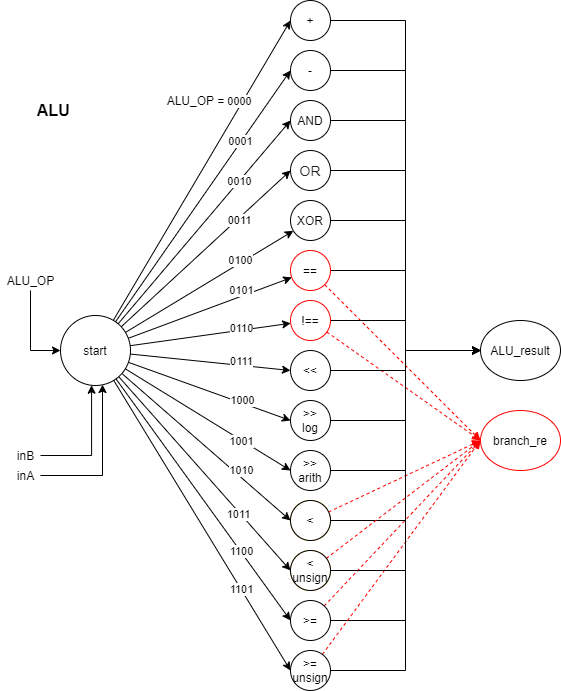
\includegraphics[width=\textwidth]{ALU.png}
	\caption{ALU operations}
	\label{fig:alu}
\end{figure}

\subsection{Architecture and Design}
To implement the ALU, it is required to have the data inputs as well as clock input and a control signal consisting of 4 bits to specify the required operation to be performed. Since there are instructions that require a branch response to know whether the next instructions shall be skipped or not, the ALU needs an additional output called \textit{branch\_re} other than the result output of the arithmetic/logical operation. The architecture of the ALU is shown in figure \ref{fig:alu_arch}:
\begin{figure}[H]
	\centering
	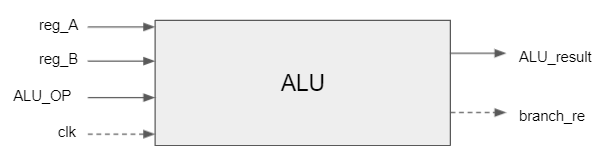
\includegraphics[width=\textwidth]{alu_arch.png}
	\caption{ALU operations}
	\label{fig:alu_arch}
\end{figure}
Not only the instructions e.g. \textit{ADD, SUB, XOR...} require an arithmetic operation but also \textit{LOAD, STORE..} require an ALU action. While \textit{ADD, SUB, XOR...} require an operation between the two input values (either register-register or register-immediate) to get a mathematical or logical result, the \textit{LOAD, STORE...} instructions require the ALU to build the target addresses for the memory access.
\subsection{Implementation}
The implementation of the ALU is based on figure \ref{fig:alu} and performs a switch-case on all the different input values of \textit{ALU\_OP}. The 4-bit input variable specifies the operation based on following declarations:
\begin{table}[H]
\setlength\arrayrulewidth{2pt}
\centering
	\begin{tabular}{|c|c|}
		\hline
		\rowcolor{light-gray}
		\textbf{ALU\_OP} & \textbf{Operation} \\
		\hline
		0000 & ADD \\
		\hline
		0001 & SUB \\
		\hline
		0010 & AND \\
		\hline
		0011 & OR \\
		\hline
		0100 & XOR \\
		\hline
		0101 & EQUAL \\
		\hline
		0110 & NEQUAL \\
		\hline
		0111 & shift\_left \\
		\hline
		1000 & shift\_right \\
		\hline
		1001 & shift\_right (arithmetic) \\
		\hline
		1010 & <\\
		\hline
		1011 & < (unsigned) \\
		\hline
		1100 & $\geq$ \\
		\hline
		1101 & $\geq$ (unsigned) \\
		\hline
	\end{tabular}
\label{aluop}
\caption{Input code and respective operation}
\end{table}
To visualize the implementation, a part of the VHDL code is displayed in the following. The case statement is based on the input \textit{alu\_op}. The ALU then performs the corresponding operation with the two inputs \textit{in\_a and in\_b}.\clearpage

\begin{lstlisting}[style=vhdl, caption=ALU VHDL code]
begin
	process(in_a, in_b, alu_op)
	begin
	--default output is 0
	branch_re <= '0';
	alu_result <= "00000000000000000000000000000000";	
		case alu_op is	
			when "0000" =>--"ADD"	
				alu_result <= in_b + in_a;	
			when "0001" =>--"SUB"	
				alu_result <= in_b -in_a;	
			when "0010" =>--"AND"	
				alu_result <= in_b AND in_a;
			when "0011" =>--"OR"
				alu_result <= in_b OR in_a;
			when "0100" =>--"XOR"
				alu_result <= in_b XOR in_a;
			when "0101" =>--"EQUAL"	
				if(in_b = in_a) then
				branch_re <= '1';
				else
				branch_re <= '0';
				end if;
	...
\end{lstlisting}
In case the operation determined by \textit{alu\_op} might be originating of a branch instruction, the \textit{branch\_re} flag has to be set respectively (line  19). Since the branch instructions only include some of the arithmetic and logical operations of the ALU, the default value for the \textit{branch\_re} is set as \textit{0}.

\clearpage
\section{\acf{RF}}
A register is a small memory element with high read and write speeds. It is therefore often used inside digital circuits to store data locally. In the case of a processor core, the total data stored in all registers specifies the machine state.\\
If the contents of each register are saved to some arbitrary memory the current state of the core can later be restored by loading this data to the corresponding registers. \\
The RISC-V unprivileged specification specifies 32 32-Bit general purpose register for the RV32I base instruction set \cite{riscv:unprivileged}.
To configure the core as well as storing status and general information about it multiple \acf{CSR} are introduced by the RISC-V privileged specification \cite{riscv:privileged}.\\
EDRICO implements both, all 32 32-Bit integer general-purpose registers as well as a selection of required \acp{CSR}.

\subsection{Architecture and Design}
A requirement for the Register Files is to allow access on one input data bus and two output data bus, each with a size of 32-Bit respectively. Multiple control signals can be accessed to control the data flow through the module. Registers are read asynchronously, hence a read operation is not dependent on any clock. Writes to a register are performed on a falling clock edge.\\
Some of the \acp{CSR} need to provide their contents to other modules without using one of the two designated output buses. This decreases unnecessary overhead on e.g. load and store operations. \\
Figure \ref{fig:RF_arch} depicts the architecture of the Register File module.

\begin{figure}[H]
	\centering
	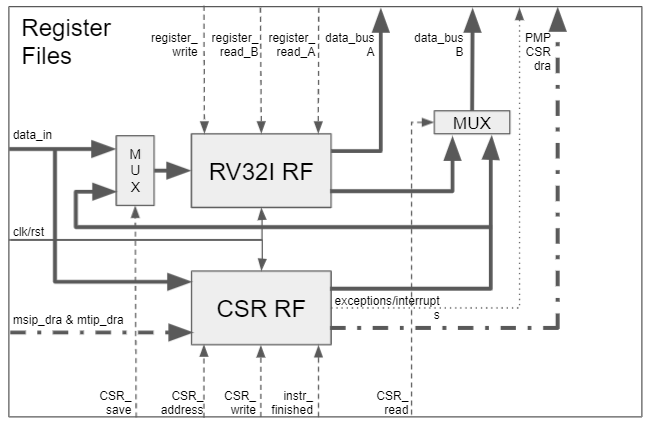
\includegraphics[width=\textwidth]{RF_arch.png}
	\caption{Register Files architecture}
	\label{fig:RF_arch}
\end{figure}

In order to write data to a register, the value needs to be put on the \textit{data\_in} bus and the corresponding control signals need to be configured. Data can be read either via the \textit{data\_busA} or \textit{data\_busB}, the CSR registers can only be accessed on \textit{data\_busB} via a MUX controlled by the \textit{CSR\_read} signal. If the bit is set, the CSR specified by \textit{CSR\_address} will be visible on \textit{data\_busB} at the next rising clock edge.\\
In order to store data to a CSR register, it has to be put on the \textit{data\_in} bus. If the \textit{CSR\_write} bit is set, the data is saved to the register specified by \textit{CSR\_address} on the next falling clock edge.\\
Execution of special \ac{CSR} instructions, like the Atomic Read/Write CSRRW \cite{riscv:unprivileged}, requires writing to both a general-purpose RV32I register and a \ac{CSR}. Since the control signals are not allowed to change during execution, it is mandatory to allow the \ac{CSR} \ac{RF} to write directly to the \ac{RV32I} \ac{RF} without utilizing the \textit{data\_in} bus.
In order to do so, the \textit{CSR\_save} signal is added to design. 
If it is applied, the \ac{CSR} Register File output is connected to the data input bus of the general purpose registers.  \\
Some of the \ac{CSR} allow direct memory accesses. These are implemented in a separate module, including the \textit{mtime}, \textit{mtimecmp} and \textit{msip} registers as well as a dedicated AXI4-Lite slave interface. To set the software and timer interrupt pending bits (which are caused by the memory mapped \ac{CSR}), the \textit{msip\_dra} and \textit{mtip\_dra} inputs are implemented.\\
The \ac{CSR} Register File is accessed by a 12 Bit addresses, \ac{RV32I} registers are accessed using a four byte address signal for each data bus, respectively.   
\subsubsection{General Purpose Registers}
The general purpose registers are used to store the data on which operations are performed on. Since RISC-V is a load-store architecture no data from the memory can be modified directly without loading it to a \ac{GPR} first (except when using atomic operations) \cite{riscv:unprivileged}.\\
Figure \ref{fig:gppr} shows the design of \ac{RV32I} Register File:
\begin{figure}[H]
	\centering
	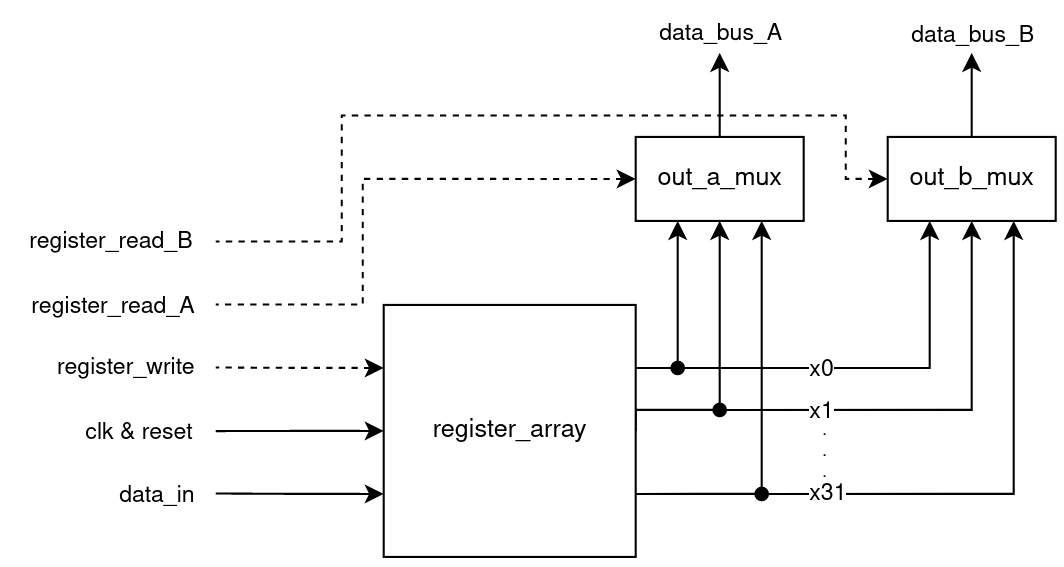
\includegraphics[width=\textwidth]{RV32I_new.png}
	\caption{General Purpose Registers}
	\label{fig:gppr}
\end{figure}
Every register may be modified via \textit{data\_in} and read via \textit{data\_busA} and \textit{data\_busB}.
The only limitation is \textit{x0}, per definition \textit{x0} must be hardwired to zero. Writing to the register is allowed but has no effect, reading will return \textit{0x00000000}.
According to the RV32I programmers model some of the other registers should be
used for dedicated purposes, like the stack pointer. There are no hardware checks
implemented in order to enforce those rules.\\
Writes are executed on a falling edge if the corresponding \textit{register\_write} signal is high. Reads are performed on a rising edge if the corresponding \textit{register\_read\_A/B} is high. There are no hardware checks implemented to prevent multiple registers from writing to the same data bus at the same time. This must be prevented by the controlling element e.g. the control unit.\\
All registers are cleared to \textit{0x00000000} on reset.
\subsubsection{\acf{CSR}}
CSRs are Control and Status Registers that are introduced to the design by the
RISC-V privileged specification. Some of the values stored inside the CSRs need to
be provided to the Exception Unit and the PMP \& PMA checker to decrease
complexity, some of that accesses can be performed through direct memory access.
Some of the CSRs are memory mapped. Memory mapped means they need to be
accessible via the system bus by any AXI4-Lite master. In order to implement this,
an AXI4-Lite salve module implementing all memory mapped CSRs is added to the
design.\\
Further Information about this module can be found in the chapter \ref{axi4slave}.
The CSRs that provide direct access are:
\begin{itemize}
	\item \textit{msip} and \textit{mtip} bits in the \textit{mpi} register (write)
	\item \textit{pmpcfg} (read)
	\item \textit{pmpaddress} (read)
\end{itemize}

Some registers are specified as WARL registers, meaning anything can be written to
them, but the value returned on read must be a legal value. Table \ref{table:csr} displays every non memory mapped CSR, the corresponding address, type, access possibility, width and a short description:
\begin{table}[H]
\setlength\arrayrulewidth{2pt}
\resizebox{\textwidth}{!}{
	\begin{tabular}{|>{\columncolor{light-gray}}l|>{\color{dark-green}}l|>{\color{dark-green}}l|>{\color{blue}}l|>{\color{red}}l|l|}
		\hline
		\rowcolor{light-gray}
		\textbf{register} & \color{black}\textbf{address} & \color{black}\textbf{type} & \color{black}\textbf{access} & \color{black}\textbf{width} & \textbf{description} \\
		\hline
		misa & 0x301 & WARL & R & 32-bit & describes supported ISAs \\
		\hline
		mvendorid & 0xF11 & N/A & R & 32-bit & describes vendor id
 \\
		\hline
		marchid & 0xF12 & N/A & R & 32-bit & describes architecture ID \\
		\hline
		mimpid & 0xF13 & N/A & R & 32-bit & describes implementation ID \\
		\hline
		mhartid & 0xF14 & N/A & R & 32-bit & describes hart id \\
		\hline
		mstatus & 0x300 & N/A & R/W & 32-bit & reflects \& controls a hart’s
		current operating state \\
		\hline
		mtvec & 0x305 & N/A & R/W & 32-bit & holds trap vector configuration \\
		\hline
		mie & 0x304 & N/A & R/W & 32-bit & reflects interrupt enable state \\
		\hline
		mip & 0x344 & N/A & R & 32-bit & holds interrupt pending bits \\
		\hline
		mcycle & 0xB00 & N/A & R/W & 64-bit & holds count of clock cycles \\
		\hline
		minstret & 0xB02 & N/A & R/W & 64-bit & holds count of executed
		instructions \\
		\hline
		mhpcounter(3-31) & 0xB03-0xB1F & N/A & R/W & 32-bit & holds count of events (lower 32
		bit) \\
		\hline
		mhpcounterh(3-31) & 0xB83-0xB9F & N/A &  & 32-bit & holds counter of events (upper
		32 bit) \\
		\hline
		mhpevent(3-31) & 0x323-0x33F & N/A & R/W & 32-bit & specifies events on which to increment corresponding
		mhpmcounter
 \\
		\hline
		mcountinhibit & 0x320 & WARL & R/W & 32-bit & controls which hardware
		performance monitoring
		counters increment \\
		& & & & & (if set, no increment) \\
		\hline
		mscratch & 0x340 & N/A & R/W & 32-bit & Dedicated for use by
		machine-mode
 \\
		\hline
		mepc & 0x341 & WARL & R/W & 32-bit & holds jump-back address during
		interrupt
 \\
		\hline
		mcause & 0x343 & N/A & R/W & 32-bit & specifies cause of
		exception/interrupt \\
		\hline
		mtval &  & N/A & R/W & 32-bit & holds information about trap \\
		\hline
		pmpcfg0-3 & 0x3A0-0x3A3 & N/A & R/W & 32-bit & Physical memory protection
		configuration
 \\
		\hline
		pmpaddr0-15 & 0x3B0-0x3BF & N/A & R/W & 32-bit & Physical memory protection
		address register \\
		\hline
	\end{tabular}}
\label{table:csr}
\caption{List of implemented CSRs}
\end{table}
\clearpage
The architecture of the CSR Register File is shown in \ref{fig:csrarch}.
\begin{figure}[H]
	\centering
	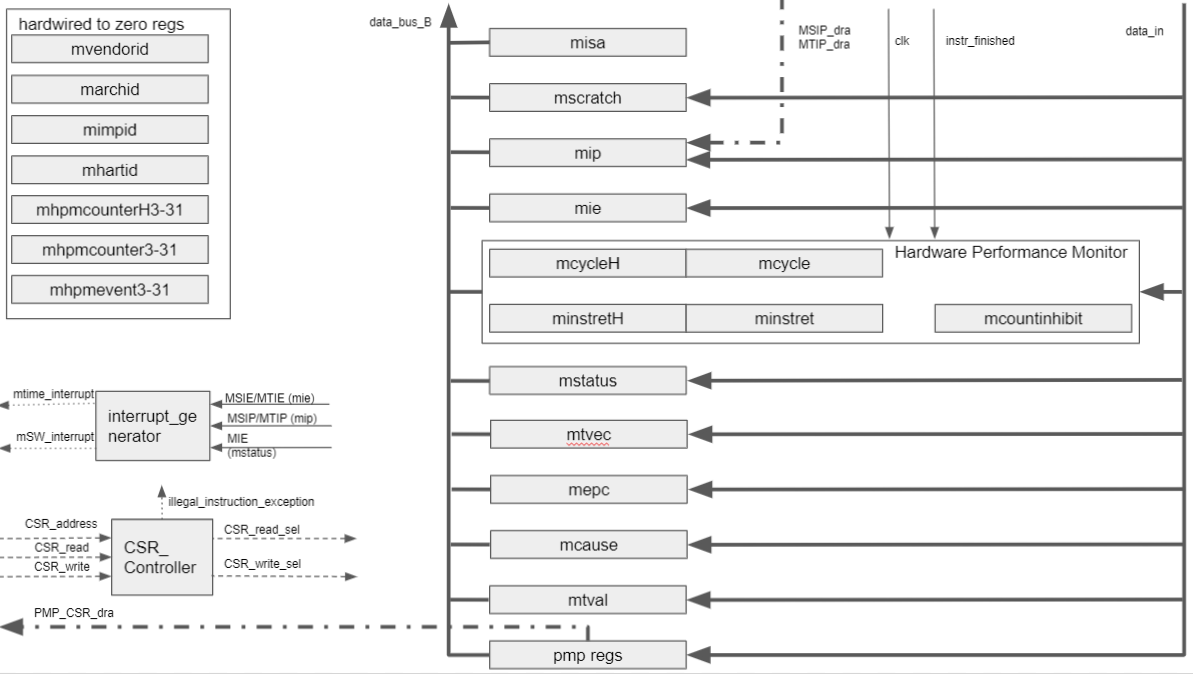
\includegraphics[width=\textwidth]{csrreg.png}
	\caption{CSR Register File Architecture}
	\label{fig:csrarch}
\end{figure}
The CSR Register File is comprised of the different CSR Registers, \textit{CSR\_Controller} and \textit{interrupt\_generator}.\\
Some of the implemented CSR registers are hardwired to zero, reads to those addresses return \textit{0x00000000} and writes have no effect if the register is defined as read only the write will result in an \textit{illegal\_instruction\_exception}. Other CSR registers may be defined as read-only. \\
The \textit{CSR\_Controller} checks if a CSR access is allowed and produces access signals for each register from the given address. If an address is not writable but yet a write is requested, the \textit{CSR\_Controller} raises an \textit{illegal\_instruction\_exception}.\\
The \textit{interrupt\_generator} checks if an interrupt is pending, enabled and if interrupts are globally enabled. In that case the corresponding interrupt is raised. The interrupts remain pending, as long as the corresponding direct register access signals it. To prevent the machine from being stuck in the interrupt, the programmer of the \ac{ISR} must clear the pending interrupts, e.g. the timer interrupt by writing to the memory mapped CSRs.\\
Some registers have special functionalities. The Hardware Performance Monitor for example counts the number of clock cycles as well as the number of executed instructions. Calculation of the \ac{CPI} can be performed as shown in \eqref{eq:CPI}:

\begin{align}
	CPI=\frac{mcycleH>>32+mcylce}{minstretH>>32+minstret}\label{eq:CPI}
\end{align}

During Benchmarks these registers can be used to calculate the performance of the core.\\
For physical memory protection, several attributes such as read and write can be specified inside the \ac{PMP} \ac{CSR}, a more detailed description of these specific registers can be found in: \cite{riscv:privileged}.\\
There are 16 \textit{pmpaddr} and four \textit{pmpcfg} registers. In order to verify that a memory access does not violate any \ac{PMP} rules, the PMP and PMA checker needs access to these registers. Performing this accesses over the \textit{data\_out\_B} bus would result in 16+4 data transfers, so 20 register accesses in total. This would impose a significant overhead of at least 20 clock cycles on every memory access. To reduce the effect of checking the \ac{PMP} rules a direct register access is implemented. 
\subsection{Implementation}
Implementing the \ac{RV32I} \ac{RF} is done by defining an array of 32 \textit{std\_logic\_vector} of 32-Bit each. The zeroth element in the array corresponds to the x0 register, therefore it can not be written and is hardwired to zero.\\
On a write, the 5-Bit \textit{register\_write} signal is used to index the corresponding array element. This is only possible since writes to the x0 register do not effect the state of the machine. Hence, no writes are performed if the write signal is set to \textit{0b00000}.\\
Since some \ac{CSR} have additional features they need to be implemented individually, therefore the matrix approach used for the \ac{RV32I} register files can not be taken. There are multiple registers that are hardwired to zero, they are implemented as one and the read write multiplexers access the same register if an access to one of these registers occurs.\\
To safe resources all \ac{CSR} implement just the bits that are needed, the others are hardwired to zero. The following listing illustrates this concept, using the \textit{mstatus} register as an example, figure \ref{fig:mstatus} shows the mstatus register according to \cite{riscv:privileged}:

\begin{figure}[H]
	\centering
	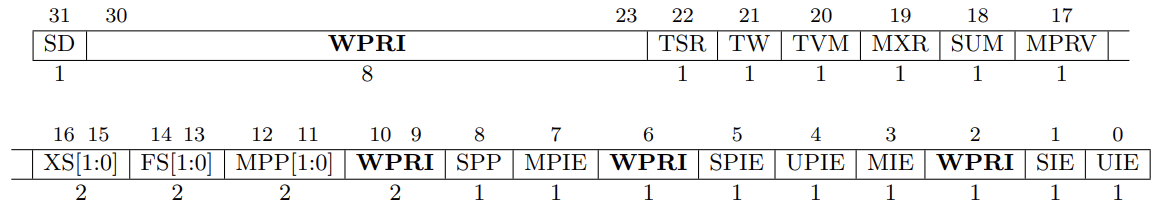
\includegraphics[width=\textwidth]{mstatus.png}
	\caption{32-Bit machine mode register (\textit{mstatus}) \cite{riscv:privileged}}
	\label{fig:mstatus}
\end{figure}

\begin{lstlisting}[style=vhdl, caption=mstatus implementation]
	---------------------------------------------------------
	--mstatus register
	---------------------------------------------------------
	mstatus_proc: process(reset, clk)
	begin
	if(reset = '1') then
	mstatus_reg <= (others => '0');
	elsif(clk'event and clk = '0' and write(0) = '1') then
	mstatus_reg <= data_in(7) & data_in(3);
	end if;
	end process;
	
	mstatus <= x"000018" & mstatus_reg(1) & "000" & mstatus_reg(0) & "000";
\end{lstlisting}

For the chosen implementation only two bits in the status register are relevant, \ac{MPIE} and \ac{MIE}. Every Other bit can be hardwired to a specific value. Since neither supervisor nor user mode are implemented are the corresponding (prior) interrupt enable bits tied to zero. The \textit{xPP} fields hold the previous privilege mode in which the machine was prior to a trap. Only machine mode is implemented, hence \ac{MPP} can be hardwired to "11" and \ac{SPP} to "00". According to \cite{riscv:privileged} all other bits may be hardwired to zero if only machine mode is implemented. \\
\clearpage
\section{PMP and PMA Checker}
Physical memory protection and attribute checking must be done in
order to ensure that only allowed and defined memory regions are accessed, providing
minimum of security and preventing the core from accessing not defined regions, which
may result in the core getting stuck.\\


\subsection{Architecture and Design}
An overview of the \ac{PMP} \& \ac{PMA} Checker is illustrated by \ref{fig:pmparch}:

\begin{figure}[H]
	\centering
	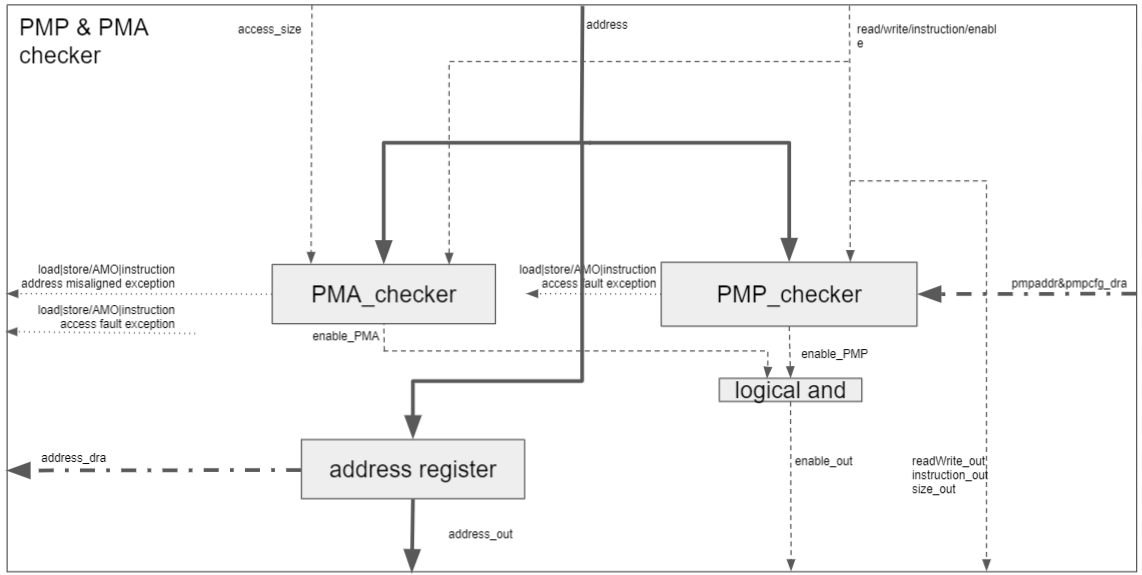
\includegraphics[width=\textwidth]{pmparch.png}
	\caption{PMP \& PMA Checker Architecture}
	\label{fig:pmparch}
\end{figure}

The \textit{PMP\_checker} is used to define memory regions and enforce several rules onto
those, for example if instructions may be fetched from a region or if writes are
allowed. In order to apply the rules the corresponding region must be locked by
setting the L-bit inside the corresponding \textit{pmpcfg} \ac{CSR}. Once locked, regions may only be unlocked by a system reset. After a restart every region is unlocked and
reset, e.g. a boot loader could enforce several rules for memory accesses in M-Mode before control hand-over to the main software running on the core. If a \ac{PMP} entry is not locked, every memory access that matches this address space succeeds.
\\
In order to specify, if reads, writes or instruction fetches are possible to a certain address, it needs to be specified inside the \textit{pmpaddr} and corresponding \textit{pmpcfg} CSRs. If an address is not specified every access is allowed, as long as the hart operates in machine mode. The PMP unit has direct access to those and enforces the rules. Figure \ref{fig:pmpaddr} and \ref{fig:pmpcfg} show these two registers.\\

\begin{figure}[H]
	\centering
	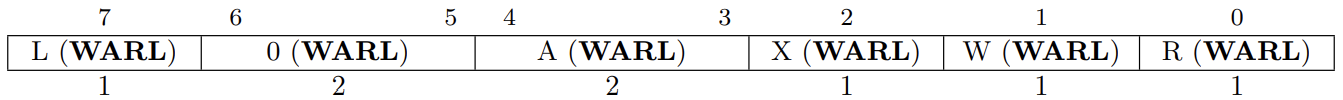
\includegraphics[width=\textwidth]{pmpcfg.png}
	\caption{8 Bit from 32-Bit \textit{pmpcfg} register \cite{riscv:privileged}}
	\label{fig:pmpaddr}
\end{figure}


\begin{figure}[H]
	\centering
	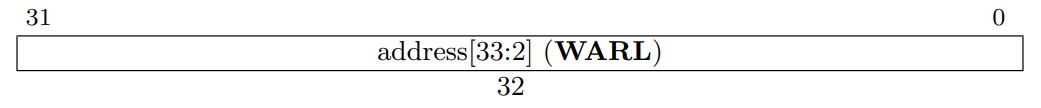
\includegraphics[width=\textwidth]{pmpaddr.png}
	\caption{\textit{pmpaddr} register \cite{riscv:privileged}}
	\label{fig:pmpcfg}
\end{figure}

One \textit{pmpcfg} register is comprised of four 8-bit configuration fields, one of which is shown in \ref{fig:pmpcfg}. The X, W and R bit specify whether or not the region defined by this entry is fit for instruction accesses, reads or writes. The size and range of the region is specified by the mode chosen by setting the A field in the configuration register. It can be configured to disable the region, specify it as \ac{TOR}, \ac{NA4} or \ac{NAPOT}. \\
If the configuration is set to \ac{TOR}, the memory region to be checked is built from the next lower \textit{pmpaddr} register (or \textit{0x00000000} for \textit{pmpcfg0}) to the corresponding address register.\\
For a \ac{NA4} region, the \textit{pmpaddr} bits 31 to 0 have to be equal to the address bits 33:2 of the address to be checked. Since \ac{EDRICO} implements an address space of only 32 bits the upper two bits are ignored. \ac{NAPOT} and \ac{NA4} regions are very similar, in fact a \ac{NA4}
region is just a 4-byte \ac{NAPOT} region \cite{riscv:privileged}. Possible sizes are $2^{x}$, with x = 32 being the maximum for this implementation. To check if an address fits in the \ac{NAPOT} range, the lower x bits of it must match the address specified in the corresponding \textit{pmpaddr} register. \\
It is important to mark that both the lower and upper address of a memory access have to be defined in the same \textit{pmpregion} in order to match it. If multiple entries match, the lower order entry wins.

Only one \ac{PMA} check is performed on memory access, to ensure that the address is aligned. A word is 32-bit, half-word 16-bit and byte 8-bit. The smallest addressable data unit is one byte long. Therefore a word access is aligned, if the memory address modulo 4 is 0 (two \acp{LSB} are zero), for a half-word access the memory address modulo 2 must be zero (\ac{LSB} is zero) and byte accesses are allowed on every address.
\\
Both checker (\ac{PMP} and \ac{PMA}) need information about the type of access (size, read/write, instruction) this is provided by the control unit. \ac{PMP} and \ac{PMA} checks
are applied on the data present as soon as the enable signal is applied. Both checks
are simple logical functions and must be performed under a clock cycle. The address
register is updated with the corresponding address after every check, independent of
its result. This must be done since the Exception Control needs access to the faulty
address at the rising clock edge if an exception is risen.
\\
Figure \ref{fig:pmpChecker} shows the design of the \textit{PMP\_checker} module:

\begin{figure}[H]
	\centering
	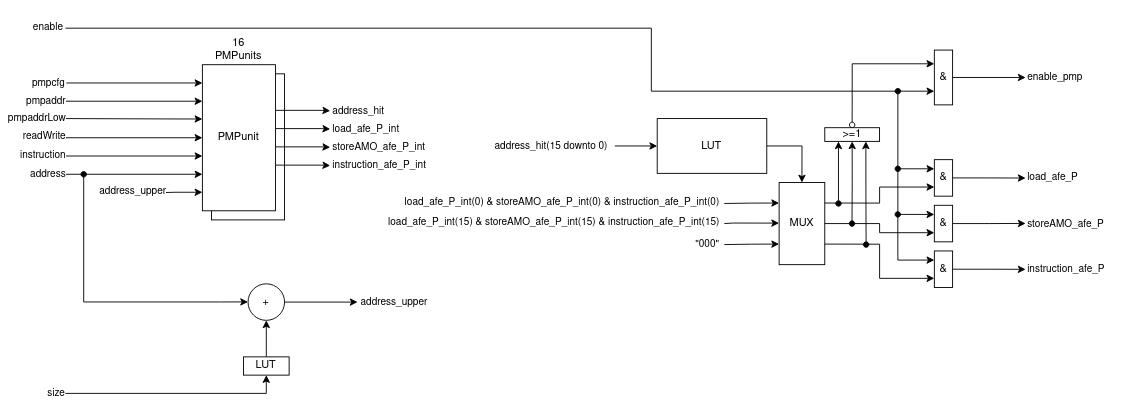
\includegraphics[width=\textwidth]{pmp_checker.png}
	\caption{\textit{pmp\_checker} module design}
	\label{fig:pmpChecker}
\end{figure}

To increase performance, all 16 \ac{PMP} checks are performed in parallel using 16 \ac{PMP} units. The results are four 16-bit vectors, to indicate an address or exception hit. For an exception to be valid, the corresponding \ac{PMP} entry must also raise an address hit. \\
The \ac{LUT} chooses the lowest order \ac{PMP} region matching the address and switches the multiplexer accordingly. 

\subsection{Implementation}
The implementation of the \textit{PMA\_checker} is relatively simple. A simple multiplexer chooses whether or not an intern enable signal is set or not, depending on the lower to bits of the address and the size of the transfer. The enable output is connected to the intern enable signal as soon as the enable input is set. A simple and gate is used to connect the intern signal with the external one. \\
The following listing shows how the access misaligned exception signals are generated inside the \textit{PMA\_checker}:

\begin{lstlisting}[style=vhdl, caption=access misaligend exception generation]
	load_ame_P <= not enable_int and enable and not readWrite;
	storeAMO_ame_P <= not enable_int and enable and readWrite;
	instruction_ame_P <= not enable_int and enable and instruction;
\end{lstlisting}

In order to perform the \ac{PMP} checks inside a \textit{PMP\_unit}, the size of a possible \ac{NAPOT} region has to be determined. A simple \ac{LUT} does the trick. Table \ref{table:NAPOT} shows its configuration:

\begin{table}[H]
	\setlength\arrayrulewidth{2pt}
	\centering
	\begin{tabular}{|>{\columncolor{light-gray}}l|l|}
		\hline
		\rowcolor{light-gray}
		\textbf{register} & \textbf{value} \\
		\hline
		pmpaddr & NAPOT\_size \\
		\hline
		XXXXXXXXXXXXXXX0 & 3 \\
		\hline
		XXXXXXXXXXXXXX01 & 4 \\
		\hline
		XXXXXXXXXXXXX011 & 5 \\
		\hline
		... & ... \\
		\hline
		XX011111111111111111 & 32 \\
		\hline
		X0111111111111111111 & 32 \\
		\hline
		01111111111111111111 & 32 \\
		\hline
		11111111111111111111 & 32 \\
		\hline
	\end{tabular}
	\label{table:NAPOT}
	\caption{\ac{LUT} to determine the size of a \ac{NAPOT} region}
\end{table}

Using the generated \ac{NAPOT} size, the address can be checked according to the flow chart depicted in figure \ref{fig:pmpunitFLOW}:

\begin{figure}[H]
	\centering
	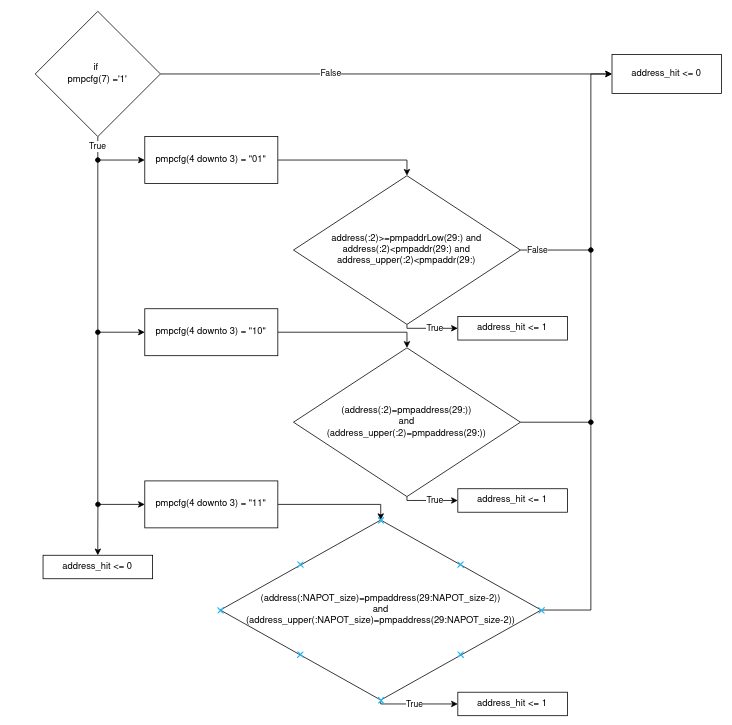
\includegraphics[width=\textwidth]{pmpUnit.png}
	\caption{\textit{pmp\_unit} flow chart for address hit detection}
	\label{fig:pmpunitFLOW}
\end{figure}

The address hit is only detected, if the \ac{PMP} entry is locked. Using the A field inside the corresponding \textit{pmpcfg} register, different scenarios are checked for an address hit. Afterwards, the exception signals for each \ac{PMP} region is generated, similar to the exception generation inside the \textit{PMA\_checker}.


\clearpage
\section{Exception Control}
The Exception Control Unit is used to guard exception entries and exits. Its
tasks are to modify the \ac{PC} accordingly, save the old \ac{PC} as well as information about the exception.
In addition, two interrupt entries are guarded by the unit. A list of all supported
exceptions and interrupts is listed below:\\\\

Exceptions can be caused by the following modules:
\begin{itemize}
	\item Control Unit
	\item \ac{CSR} register file
	\item \ac{PMP} \& \ac{PMA} checker
	\item \ac{AXI4-Lite} Master
\end{itemize}


The Control Unit may cause the following exceptions:
\begin{itemize}
	\item illegal instruction exception
	\item breakpoint exception
	\item environment-call-from-M-mode exception
\end{itemize}

The \ac{PMP} \& \ac{PMA} checker may cause the following exceptions:
\begin{itemize}
	\item load access fault exception
	\item store/\ac{AMO} access fault exception
	\item instruction access fault exception
	\item load address misaligned exception
	\item store/\ac{AMO} address misaligned exception
	\item instruction address misaligned exception
\end{itemize}

The \ac{CSR} register file may cause the following exceptions/interrupts:
\begin{itemize}
	\item timer interrupt
	\item software interrupt
	\item illegal instruction exception
\end{itemize}

The \ac{AXI4-Lite} Master may cause the following exceptions
\begin{itemize}
	\item load access fault exception
	\item store/\ac{AMO} access fault exception
	\item instruction access fault exception
\end{itemize}

\subsection{Architecture and Design}
Figure \ref{fig:EC} shows the architecture of the Exception Control:
\begin{figure}[H]
	\centering
	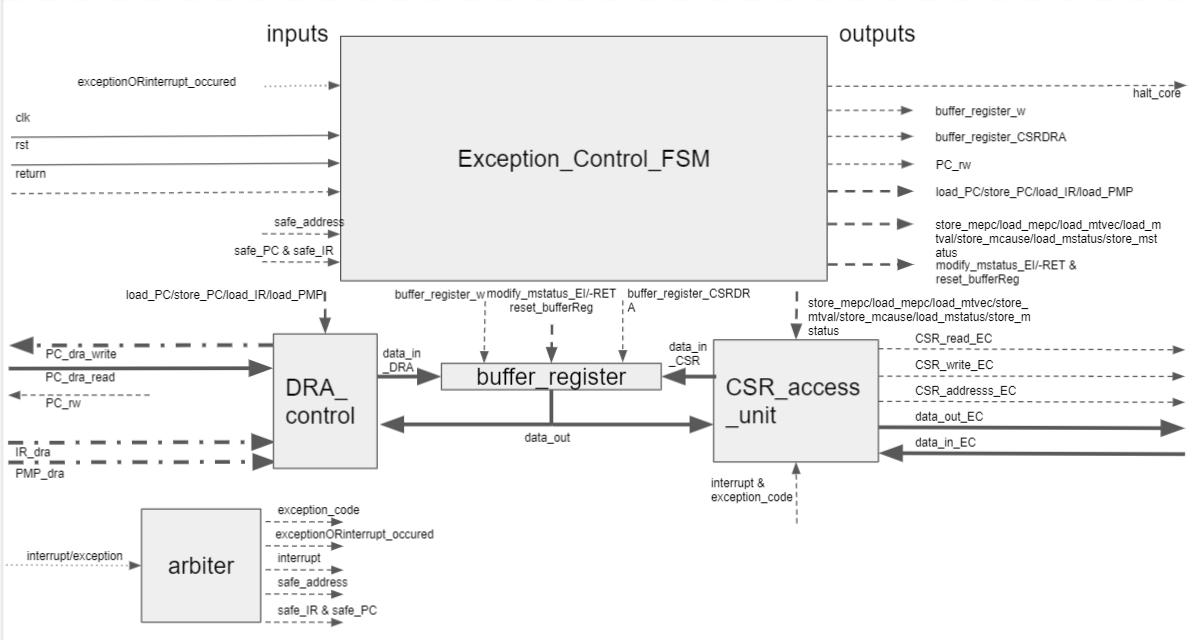
\includegraphics[width=\textwidth]{EC.png}
	\caption{Exception Control Architecture}
	\label{fig:EC}
\end{figure}
The Exception Control module is comprised of a \ac{FSM} and an arbiter to decide if an
interrupt or exception is taking place and which one shall be handled if multiple are raised at a time. To modify registers a \textit{DRA\_control} as well as a \textit{CSR\_access\_unit} and a buffer register are added to the design. 
The \textit{DRA\_control} module is used to load the Instruction Register, PMP address register and Program Counter. A load to the PC may also be performed, in order to do so the \textit{PC\_rw} signals must be asserted one clock cycle earlier by the FSM.\\
The \textit{buffer\_register} is implemented to allow data shares between the \textit{DRA\_control} and \textit{CSR\_access\_unit}. It implements another functionality that allows to set either the \ac{MIE} register to 1 (trap exit) or the \ac{MPIE} register to 0 (trap entry) and switch the two bits (\ac{MIE} and \ac{MPIE}) on the \textit{data\_out} line. This feature is used to modify the \textit{mstatus} register according to \cite{riscv:privileged} in no more than two clock cycles.\\
The \textit{CSR\_access\_unit} is used to perform register accesses to the \ac{CSR} register file. During Exception entry or return the \textit{data\_bus\_B} must be connected to the
\textit{data\_in\_EC} bus and the \textit{data\_in} bus to the \textit{data\_out\_EC} bus. This is done by implementing a multiplexer at the corresponding buses controlled by the\textit{ halt\_core} signal.\\
If an exception or interrupt is raised, the following actions are performed:
\begin{itemize}
	\item write the current \textit{PC+4} to \textit{mpec}
	\item modify \textit{mcause} to reflect the cause of the exception/interrupt
	\item update \textit{mtval} to provide additional information
	\item modify \textit{mstatus} (safe \ac{MIE} to the \ac{MPIE} and set \ac{MIE} to zero)
	\item update the \ac{PC} using the value stored in \textit{mtvec}
\end{itemize}
If multiple exceptions occur at once, only the highest priority exception is taken, as specified in \cite{riscv:privileged}.\\
If an exception is raised, while the processor is in a trap, \textit{mpec}, \textit{mcause} and \textit{mtval} are overwritten. In order to avoid a large hardware register stack, saving the return address and other information stored in those registers is left to the trap handler,.\\
If an exception entry shall be performed the \textit{exceptionORinterrupt\_occured} signal on the FSM is high, if the return signal is high it indicates that an exit shall be performed, however if both signals are high the entry will be performed.
\clearpage
\subsection{Implementation}
The \textit{Exception\_Control\_FSM} is a meely \ac{FSM}. It is sensitive to the rising clock edge. The \ac{FSM} is implemented in two \ac{VHDL} processes, one synchronous to update the state and one asynchronous to generate the output signals and the next state. Figure \ref{fig:ECFSM} shows the state diagram of said \ac{FSM}:
\begin{figure}[H]
	\centering
	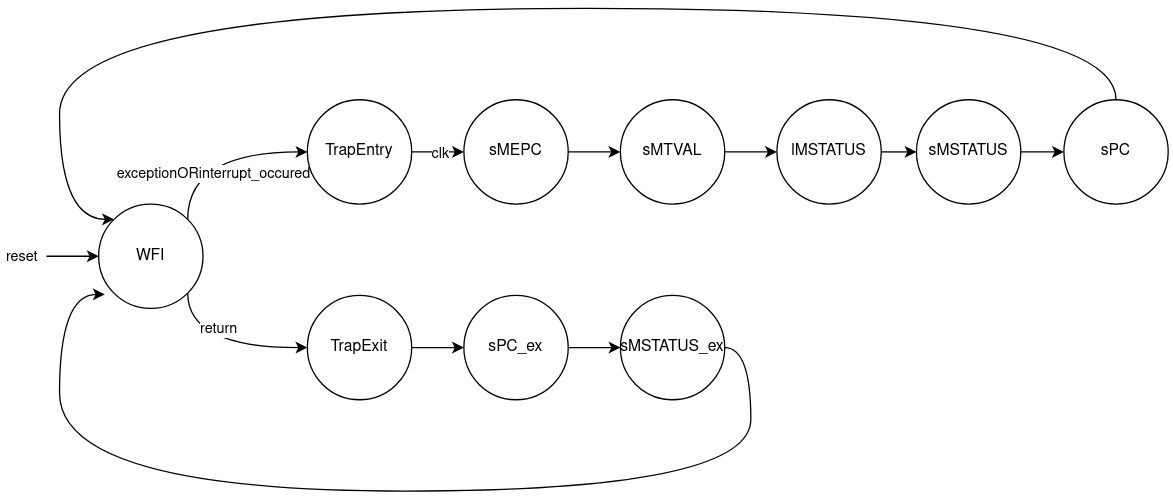
\includegraphics[width=\textwidth]{ECFSM.png}
	\caption{state diagram of the \textit{Exception\_Control\_FSM}}
	\label{fig:ECFSM}
\end{figure}
Natively the \ac{FSM} is in the \textit{WFI} state, waiting for an interrupt, exception or return to be raised. On trap entry, the upper branch of the state diagram is executed, the lower one is performed on trap exit. The \textit{halt\_core} signal is set to high, when entering either one of the branches. This stops the core and rerouts all significant control signals of the \ac{RF} to be connected to the Exception Control unit.\\
The outputs of each state can be found as a table in the appendix. 


\clearpage
\section{AXI4-Lite Master}
To connect the processor to peripherals the \ac{AXI4-Lite} protocol is used. Due to its
popularity many \acp{IP} such as \ac{BRAM} can be connected to each other using an
Interconnect. \ac{EDRICO} contains a master and a slave interface. Both of which are
explained in more detail in the following sections:
\subsection{Architecture and Design}
Three substantial building blocks are implemented to form the master interface.
Figure \ref{fig:aximaster} depicts the architecture of it:
\begin{figure}[H]
	\centering
	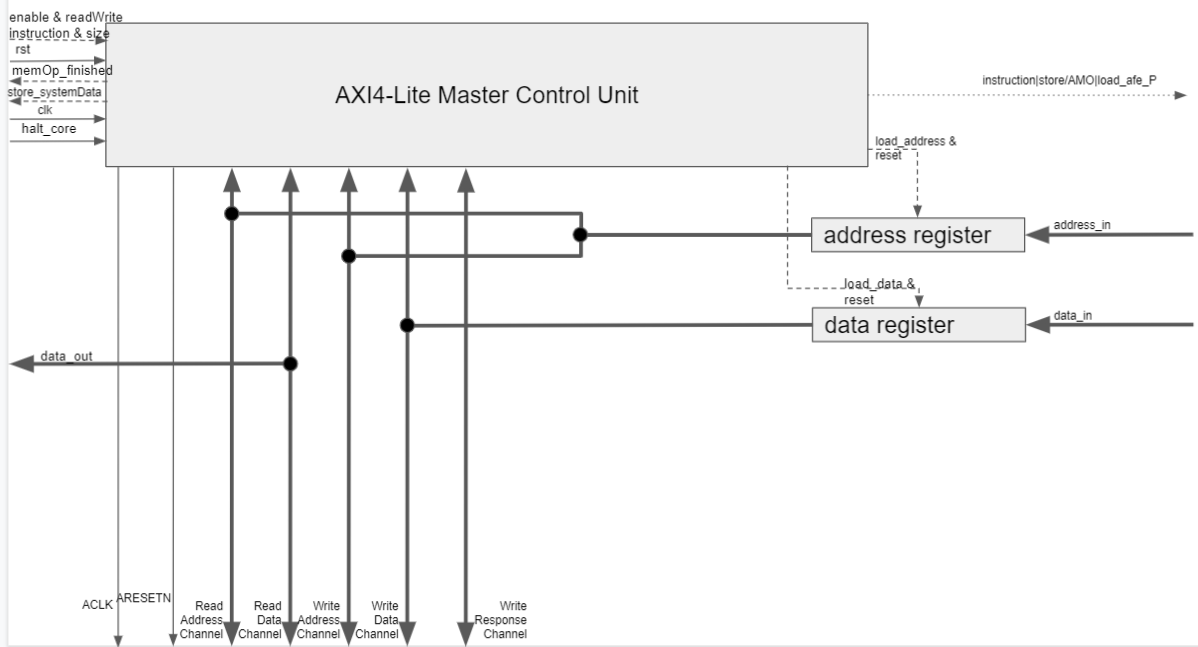
\includegraphics[width=\textwidth]{aximaster.png}
	\caption{AXI4-Lite Master architecture}
	\label{fig:aximaster}
\end{figure}
It includes two registers, for data and address. These are loaded on the rising edge of the system clock, if the corresponding load signal is applied. Both register outputs are constantly connected to the corresponding \ac{AXI} signals \textit{(AWADDR/ARADDR and WDATA)}.\\
The \textit{AXI4-Lite Master Control Unit} is in charge of controlling the \ac{AXI} transfer. It controls the ready and valid signals as well as the register reads and writes. It is clocked with \textit{M\_AXI\_ACLK}. To reset the module either the reset (active high) or \textit{M\_AXI\_ARSTN} (active low) may be applied. To start a transfer, the enable signal must be high on a rising clock edge. This will cause the corresponding registers and valid signals to be updated (see section 2.5.2 for more information on the \ac{AXI} protocol). It is mandatory, that the correct address and data values are present as soon as the enable signal is high. Otherwise a faulty transfer will be initiated, since the valid signals are set to high even though data and address are not valid yet. \\
If data is ready to be read from the system bus, it is routed to an output of the master and the \textit{store\_systemSystemData} is set to high, in order to ensure a correct read, this process shall not be clocked. The surrounding system is responsible to store the received data in the correct register.\\
At the end of a data transfer, the \textit{memOp\_finished} signal is set to high, informing the Control Unit that it can proceed operations.\\
If an error occurred during an access, the \textit{instruction\_afe\_P}, \textit{storeAMO\_afe\_P} or \textit{load\_afe\_P} exceptions are raised. And remain high until the \textit{halt\_core} signal is applied to the \textit{AXI4-Lite Master Control Unit}.
\subsection{Implementation}
As described in chapter 2 each \ac{AXI} channel implements a flow-control handshake, using a ready and valid signal. The transmitter interface applies the valid signal as soon as the signal on the corresponding channel is valid. If the receiver is ready to receive data, it ties the ready signal to high. A transfer on one channel is finished as soon as the valid and ready signal are detected to be high on a rising clock edge.\\
Figure \ref{fig:AXIhandshake} shows how the address read(right) and read data(left) handshakes are implemented on \ac{EDRICO}:

\begin{figure}[H]
	\centering
	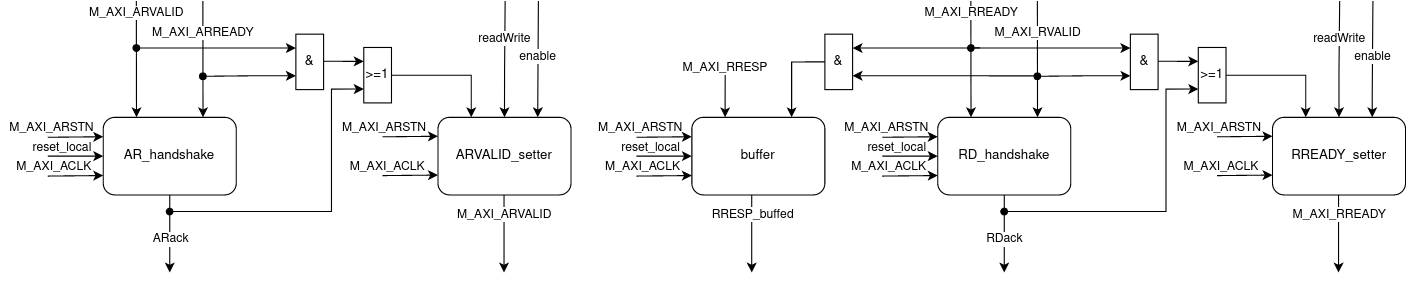
\includegraphics[width=\textwidth]{axihandshake.png}
	\caption{read handshake implementation in \textit{AXI4-Lite Control Unit}}
	\label{fig:AXIhandshake}
\end{figure}

Both handshake mechanisms work concurrent and do not interfere with one another. If a handshake is detected, the corresponding acknowledge signal (\textit{ARack; RDack}) is set to high. These acknowledge signals can only be reset by a system wide reset or a local reset initiated by the control \ac{FSM} described in the following text segment.\\
\textit{M\_AXI\_ARVALID} and \textit{M\_AXI\_RREADY} are the two handshake signals that are controlled by the implemented master. A setter controls each of these signals. If \textit{readWrite} is low and enable is high, indicating that a read transfer is started, the corresponding output signal is set. It is automatically reset as soon as the handshake is detected (on a rising clock edge). Since the output signal of the setter is part of the handshake it will de-assert its own reset signal one clock cycle later, causing an unstable valid or ready signal. To prevent this the setter reset is connected to the corresponding acknowledge signal. Guaranteeing that the signal can not be reasserted as long as the \ac{AXI} transfer is still running.\\
The read data and write response channel handshakes implement an additional block, buffering the \textit{RRESP} and \textit{BRESP} signals, respectively. Therefore allowing evaluation of the slaves response on a later stage of the transfer.\\
\\
To control the operation of the \ac{AXI} master a finite state machine is implemented. Figure \ref{fig:axifsm} depicts the corresponding state diagram:

\begin{figure}[H]
	\centering
	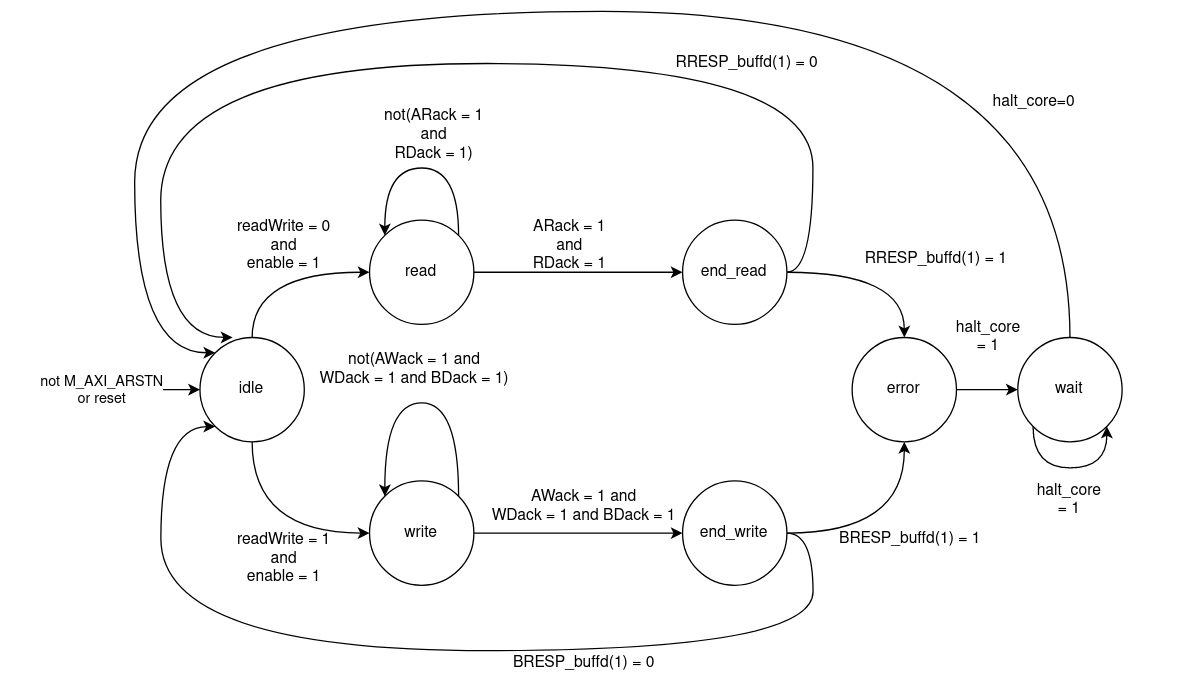
\includegraphics[width=\textwidth]{axifsm.png}
	\caption{control \ac{FSM} of the \textit{AXI4-Lite Control Unit}}
	\label{fig:axifsm}
\end{figure}

After reset, the \ac{FSM} remains in \textit{idle} state until the \textit{enable} signal is set to high. It then changes to either \textit{read} or \textit{write}, depending on the value of the \textit{readWrite} signal. The machine remains in the \textit{read/write} state until all acknowledge signals are set to high, hence all necessary handshakes are completed. Performing and detecting the handshake signals independent from the \ac{FSM} simplifies the design significantly and guarantees that the handshakes do not need to be performed in any particular order.\\
After performing all expected handshakes, the \textit{end\_read/end\_write} states are entered, these are used to check if any errors occurred during the transfer.\\
If that is the case, the \textit{error} state will be entered. The machine remains in \textit{error} state until the trap is handled by the \textit{Exception Control} unit (\textit{halt\_core} = 1). The corresponding access fault exception signals are generated, similar to the exception generation in the \textit{PMP\_checker}.\\
It then changes to \textit{wait} state until \textit{halt\_core} is deasserted and the core restarts execution. \\
\\
Some of the system control signals are generated independently from the \ac{AXI} control unit, in order to guarantee fast execution and decrease overhead introduced by the state changes inside the \ac{FSM}. The following figure shows how these are generated:

\begin{figure}[H]
	\centering
	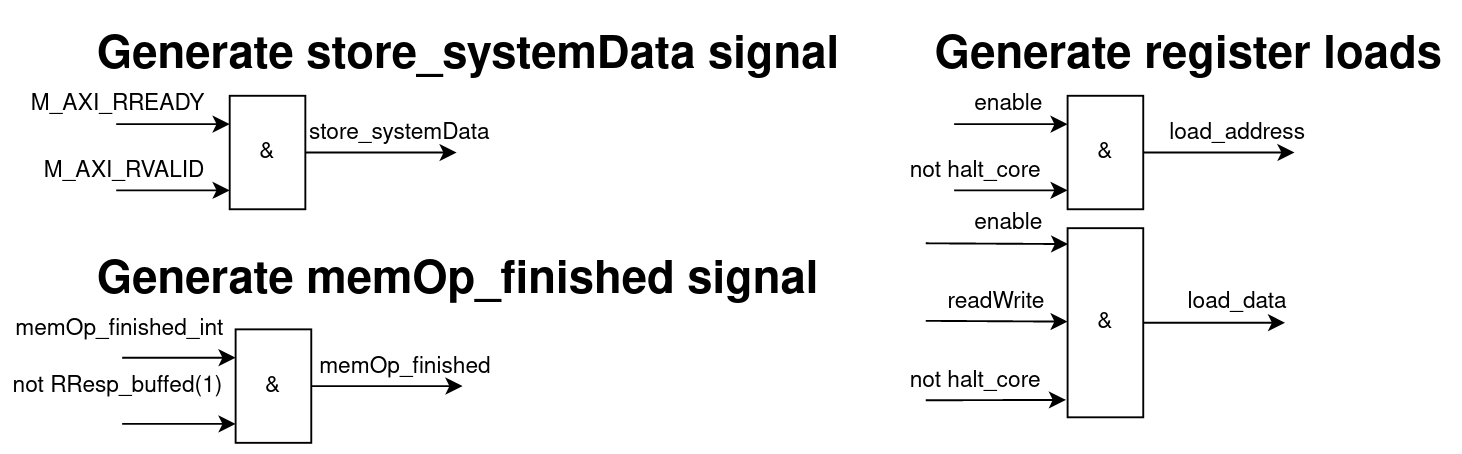
\includegraphics[width=\textwidth]{axiSysCont.png}
	\caption{Generation of system control signals inside the \textit{AXI4-Lite Control Unit}}
	\label{fig:axiSysCont}
\end{figure}

Five \ac{AXI4-Lite} signals are generated without using the FSM, in order to decrease complexity. Figure \ref{fig:axisignals} depicts the implementation of said signals:

\begin{figure}[H]
	\centering
	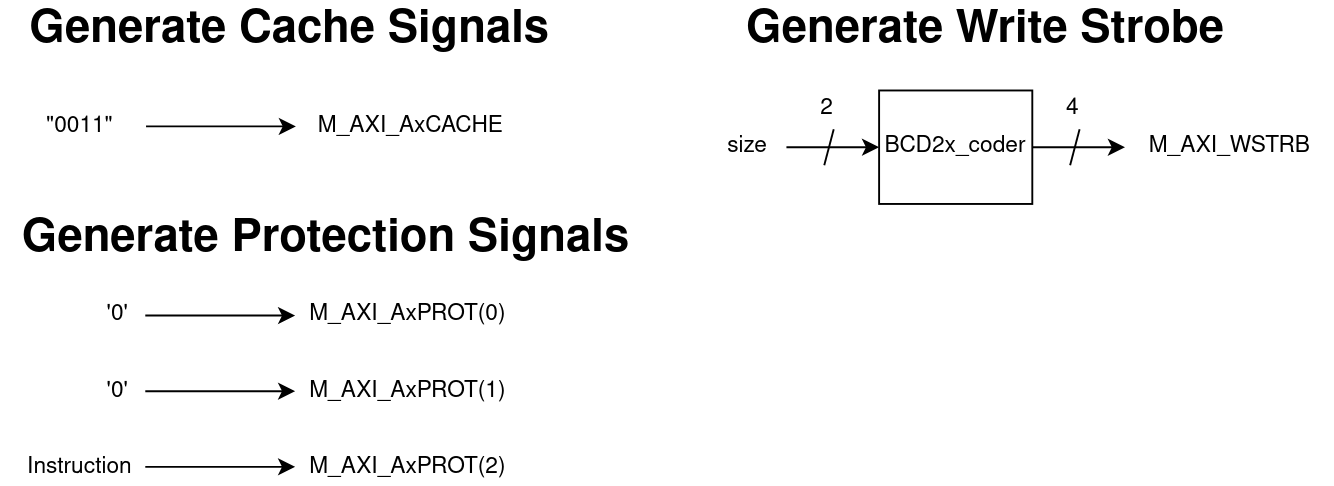
\includegraphics[width=\textwidth]{axisignals.png}
	\caption{Generation of generic \ac{AXI4-Lite} signals inside the \textit{AXI4-Lite Control Unit}}
	\label{fig:axisignals}
\end{figure}

The\textit{ M\_AXI\_AxCACHE} is hardwired to \textit{"0011"} to determine that the access is normal non-cacheable bufferable. This is specified since \ac{EDRICO} does not employ any memory consistency model. The first two bits of the protection signals are set to 0, in order to ensure that every access is secure and unprivileged since the only implemented privilege mode is machine-mode. \textit{M\_AXI\_AxPROT}(2) is adjusted, accordingly to the executed access (instruction or data).\\
\textit{M\_AXI\_WSTRB} signals what bytes of the transfer are valid to be used. For a word it is set to \textit{0x1}. for a half-word to \textit{0x3} and for a word transfer to \textit{0xF}.

\clearpage
\section{AXI4-Lite Slave}
\label{axi4slave}
Some of the RISC-V \acp{CSR} must be memory mapped, meaning the must be
accessible by other devices via the memory space. The for each \ac{CSR} is predefined,
corresponding to the \acp{CLINT} module by SiFive since this is the closest thing to an industry
standard \cite{sifive:clint}.
\begin{table}[H]
	\setlength\arrayrulewidth{2pt}
	\centering
	\resizebox{\textwidth}{!}{
	\begin{tabular}{|>{\columncolor{light-gray}}l|>{\color{dark-green}}l|>{\color{blue}}l|>{\color{red}}l|l|}
		\hline
		\rowcolor{light-gray}
		\color{black}\textbf{register} & \color{black}\textbf{address} & \color{black}\textbf{access} & \color{black}\textbf{width} & \color{black}\textbf{description}\\
		\hline
		msip & 0x0200\_0000 & R/W & 32-bit & hold software interrupt pending bit \\
		\hline
		mtimecmp & 0x0200\_4000 & R/W & 32-bit & hold time compare value (lower 32 bit) \\
		\hline
		mtimecmph & 0x0200\_0004 & R/W & 32-bit & hold time compare value (upper 32 bit) \\
		\hline
		mtime & 0x0200\_BFF8 & R/W & 32-bit & hold time (lower 32 bit) \\
		\hline
		mtimeh & 0x0200\_BFFB & R/W & 32-bit & hold time (upper 32 bit) \\
		\hline
	\end{tabular}}
	\caption{Memory Mapped CSRs}
\end{table}
\subsection{Architecture and Design}
The \ac{AXI4-Lite} slave accepts data transfers and performs the reads/writes to the
\ac{CSR}. Figure \ref{fig:axislave} shows the architecture, including the memory mapped \ac{CSR}:
\begin{figure}[H]
	\centering
	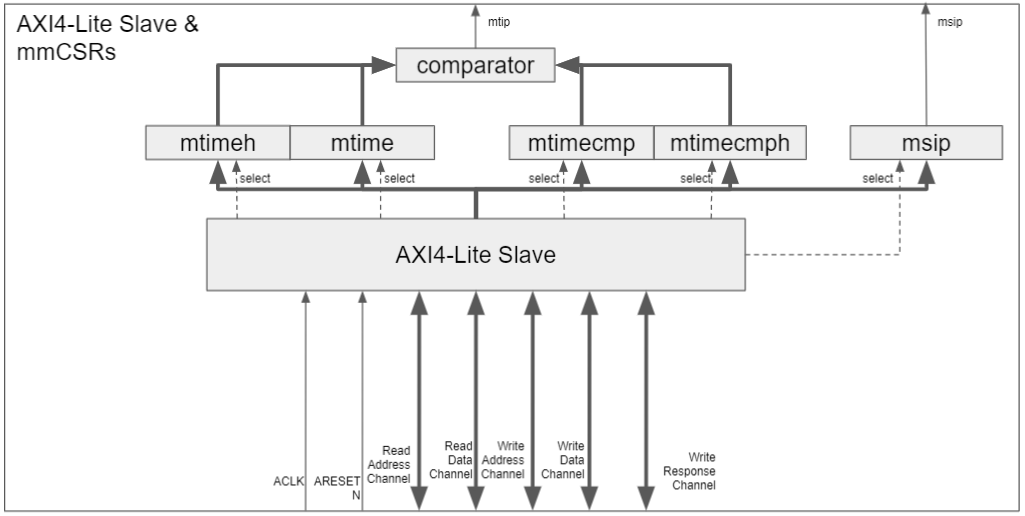
\includegraphics[width=\textwidth]{axislave.png}
	\caption{AXI4-Lite Slave Architecture}
	\label{fig:axislave}
\end{figure}
The \ac{AXI} slave allows reads and writes to the 32 bit registers \textit{mtimeh}, \textit{mtime},
\textit{mtimecmp} and \textit{mtimecmph} as well as the \textit{msip} register.\\
A comparator is used to trigger a timer interrupt. It compares \textit{mtime} and
\textit{mtimecmp}. If the value of \textit{mtime} is equal or greater than the one in \textit{mtimecmp}, the
\textit{mtip} signal is asserted.\\
The interrupt remains posted, until it is cleared by writing to the \textit{mtimecmp} register.
Writing a \textit{0xFFFFFFFF} to the \textit{msip} register causes the \textit{msip} signal to be raised. Effectively raising a software interrupt.
Table \ref{CSRreset} shows the reset values for each CSR:
\begin{table}[H]
	\setlength\arrayrulewidth{2pt}
	\centering
	\begin{tabular}{|>{\columncolor{light-gray}}l|l|}
		\hline
		\rowcolor{light-gray}
		\textbf{register} & \textbf{value} \\
		\hline
		msip & 0x00000000 \\
		\hline
		mtimeh & 0x00000000 \\
		\hline
		mtime & 0x00000000 \\
		\hline
		mtimecmph & 0xFFFFFFFF \\
		\hline
		mtimecmp & 0xFFFFFFFF \\
		\hline
	\end{tabular}
	\label{CSRreset}
	\caption{Memory Mapped CSRs reset values}
\end{table}
\subsection{Implementation}
To simplify the development of \ac{EDRICO} the \ac{AXI4-Lite} slave is implemented using the automatic \ac{AXI}4 peripheral generation workflow of Vivado. The generated 5 register salve \ac{IP} is then modified to include the comperator and to comply to the predefined address space.

